\documentclass{subfiles}
\begin{document}
\begin{figure}[h!]
    \centering
    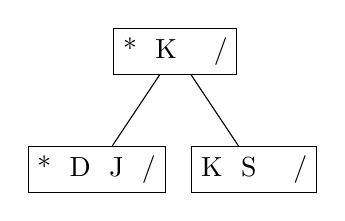
\begin{tikzpicture}[
            bNode/.style={draw=black, align=center, rectangle, minimum width=30pt, minimum height=15pt},
            every name/.style={font=\bfseries, SkyBlue4},
            sibling distance=2cm
        ]

        \node [bNode] {* \ K \ \ \ /}
        child {node [bNode, ] {* \ D \ J \ /}}
        child {node [bNode, ] {K \ S \ \ \ /}};

    \end{tikzpicture}
    \caption{Esempio di B-Tree.}
    \label{Fig:4}
\end{figure}
\end{document}